\documentclass[a4paper,12pt]{article} % тип документа

%  Русский язык
\usepackage{multirow}
\usepackage{wrapfig}
\usepackage[T2A]{fontenc}   % кодировка
\usepackage[utf8]{inputenc}   % кодировка исходного текста
\usepackage[english,russian]{babel} % локализация и переносы

\usepackage{indentfirst} %Красная строка
\usepackage[a4paper,top=1.3cm,bottom=2cm,left=1.5cm,right=1.5cm,marginparwidth=0.75cm]{geometry}
\usepackage[usenames]{color}
\usepackage{colortbl}
\usepackage{float}

\usepackage{graphicx}%картинки
\usepackage{textcomp}%Номер
\usepackage{wrapfig}%обтекание текстом теблиц и картинок
%гиперссылки
\usepackage{hyperref}
\usepackage[rgb]{xcolor}
\hypersetup{     %гипперсылки
 colorlinks=true, %false:ссылки в рамках
 urlcolor=blue   %на URL
 }
% Заметки
\usepackage{todonotes}
% Номера формул(необязятельна, см. по ситуации)
%\mathtoolsset{showonlyrefs=true} % Показывать номера только у тех формул, на которые есть \eqref{} в тексте.

% Математика
\usepackage{amsmath,amsfonts,amssymb,amsthm,mathtools} 
\usepackage{wasysym}

\usepackage{euscript} % Шрифт Евклид
\usepackage{mathrsfs} % Красивый матшрифт

\title{\textbf{Лабораторная работа. Термический анализ двухкомпонентных систем} }

\author{Алекснадров Максим, Кузнецов Роман, Тналиев Тимур \\ Б04-202}
\date{1 марта 2024}

\begin{document}

\maketitle

\section{Цель работы}
Экспериментальное исследование двухкомпонентной системы с применением метода дифференциальное сканирующей калориметрии (ДСК).
\section{Оборудование и материалы}
\begin{enumerate}
    \item Кристаллические соли $NaNO_3$ и $KNO_3$ И навески их смесей.
    \item Алюминиевые тигли с крышками
    \item Шпатели, аналитические весы
    \item ДСК термоанализатор
\end{enumerate}
\section{Введение}
\subsection{Диаграммы плавкости (T-x диаграммы)}
Для исследования фазовых равновесий «твердое-жидкость» в двухкомпонентной системе обычно используют Т—х диаграмму (диаграмму 
плавкости). Вид диаграммы плавкости будет определяться рядом факторов, 
среди которых наличие аллотропных модификаций, возможность 
образования химических соединений, способность компонентов взаимно 
растворяться: 
\begin{enumerate}
    \item Системы компонентов обладающих неограниченной растворимостью как 
в твердой, так и в жидкой фазе характеризуются наиболее простыми по 
виду диаграммами плавкости (рис. 1). 
\newpage
\begin{figure}[H]
    \centering
    \includegraphics[width = 180 mm]{image_1.jpg}
    \caption{Диаграммы плавкости двухкомпонентных систем с неограниченной}
\end{figure}
Диаграммы плавкости таких систем по виду аналогичны Т—х диаграммам 
«жидкость- пар» или «с азеотропом». 
\item Двухкомпонентные 
системы, в которых компоненты неограниченно растворимы в жидкой 
фазе, но не смешиваются в твёрдой фазе. Такие диаграммы характерны 
для большинства двухкомпонентных систем органических соединений, 
поскольку даже изомеры органических соединений редко образуют 
смешанные кристаллы. 
\begin{figure}[H]
    \centering
    \includegraphics[width = 180 mm]{image_2.jpg}
    \caption{Мольная доля изомера $В$}
\end{figure}
На рис. 2 приведены три диаграммы плавкости двухкомпонентных смесей: мета-, орто- и пара-изомеров хлорнитробензола. Их отличительной 
особенностью является наличие характерного излома на кривой ликвидуса 
(точка Е на рис. 2). 

\end{enumerate}
\subsection{Уравнение Шредера}
Допустим, что в двухкомпонентной двухфазной 
системе вещества 1 и 2 не образуют между собой твёрдого раствора, то 
полностью смешиваются в жидкой фазе (расплаве). Рассмотрим равновесие 
между одним из этих веществ, находящимся в твёрдой фазе и в расплаве, где 
его активность равна $a_i$. 
Из условия равновесия $\mu(fluid) = \mu(solid)$ следует
\begin{equation}
    {\mu_i}^{o}(fluid) + RTln{a_i}^{fluid} = {\mu_i}^{o}(solid)
\end{equation}
Выражая отсюда активность и дифференцируя обе части равенства, приходим с уравнению Шредера
\begin{equation}
     \Bigl(\frac{\partial ln{a_i}^{fluid}}{\partial T}\Bigr)_P = \frac{\Delta H_i^{o}}{RT^2},
\end{equation}
которое для идеальных растворов выглядит как 
\begin{equation}
     \Bigl(\frac{\partial ln{x_i}^{fluid}}{\partial T}\Bigr)_P = \frac{\Delta H_i^{o}}{RT^2},
\end{equation}
Здесь $\Delta H_i^{o}$ - стандартная энтальпия плавления $i$-го компонента. 
Если принять, что $\Delta H_i^{o}$ не зависит от температуры, то после интегрирования получим уравнение Шредера в интегральной форме: 
\begin{equation}
    ln{x_i}^{fluid} = -\frac{\Delta H_i^{o}}{R}\Bigl(\frac{1}{T} - \frac{1}{{T_i}^{o}}\Bigr),
\end{equation}
где ${T_i}^{o}$ - температура плавления чистого i-го компонента. 
Положение точки эвтектики (температуру Т и состав хэвт) нетрудно 
вычислить из уравнения Шредера. 
Линии ликвидуса и солидуса делят диаграмму плавкости на ряд 
областей: I - жидкий расплав; II - жидкий расплав и кристаллы компонента А; 
Ш - жидкий расплав и кристаллы компонента В; IV - механическая смесь двух 
чистых кристаллических компонентов А и В. 
Часто встречаются системы, компоненты которых частично растворимы 
в твёрдом состоянии и из расплавов кристаллизуются не чистые компоненты, 
а твёрдые растворы. При этом равнение Шредера имеет вид 
\begin{equation}
    ln\frac{{x_i}^{fluid}}{{x_i}^{solid}} = -\frac{\Delta H_i^{o}}{R}\Bigl(\frac{1}{T} - \frac{1}{{T_i}^{o}}\Bigr),
\end{equation}
Пример одной из таких диаграмм плавкости приведён на рис. 3 в 
упрощенной форме. Области II, III и V, где система является двухфазной, 
затемнены. 
\paragraph{Cхема установки}:
\begin{figure}[H]
    \centering
    \includegraphics[width = 100 mm]{ust.jpg}
\end{figure}
\begin{figure}[H]
    \centering
    \includegraphics[width = 180 mm]{image_3.jpg}
    \caption{Диаграмма плавкости двухкомпонентной смеси $NaNO_3$ и $KNO_3$}
\end{figure}
\section{Методика}
\begin{enumerate}
    \item Измерение $T$ охлаждаемой или нагреваемой смеси
    \item При изменении фазы появляются изломы
    \item Пологие линии говорят о кристализации расвтора, выделяется теплота
    \item Начало - ликвидус, конец - солидус.
\end{enumerate}
\section{Тепловой поток}
\begin{equation}
    -\Delta Q = \frac{\Delta T}{R},
\end{equation}
где $\Delta T$ разность температур между исследуемым образцом и эталоном, $R$ - тепловое сопротивление диска в ячейке. 
ДСК - метод, при котором измеряется разность тепловых потоков к исследуемому образцу и к инертному эталону.

\section{Ход работы}
\begin{enumerate}
    \item Взвесим навеску на аналитических весах.
    \begin{itemize}
        \item    m_{pot} = 52 (mg) $ - масса тигеля 
        \item    $m_{full} = m_{pot} + m_{mix} = 70.2 (mg)$ - масса полная 
        \item    $m_{mix} = 18.2 (mg)$ - масса смеси 
        
    \end{itemize}
    \item Поместим тигель с образцом и эталон.
    \item Проводим эксперимент по нагреву образца от комнатной температуры до 350 $^{\circ}C$ и охлаждаем до 200 $^{\circ}C$. Затем повторяем программу. 
    \end{enumerate}
    Были получены следующие результаты:
\begin{figure}[H]
    \centering
    \includegraphics[width = 180 mm]{image_4.jpg}
\end{figure}

 \begin{figure}[H]
    \centering
    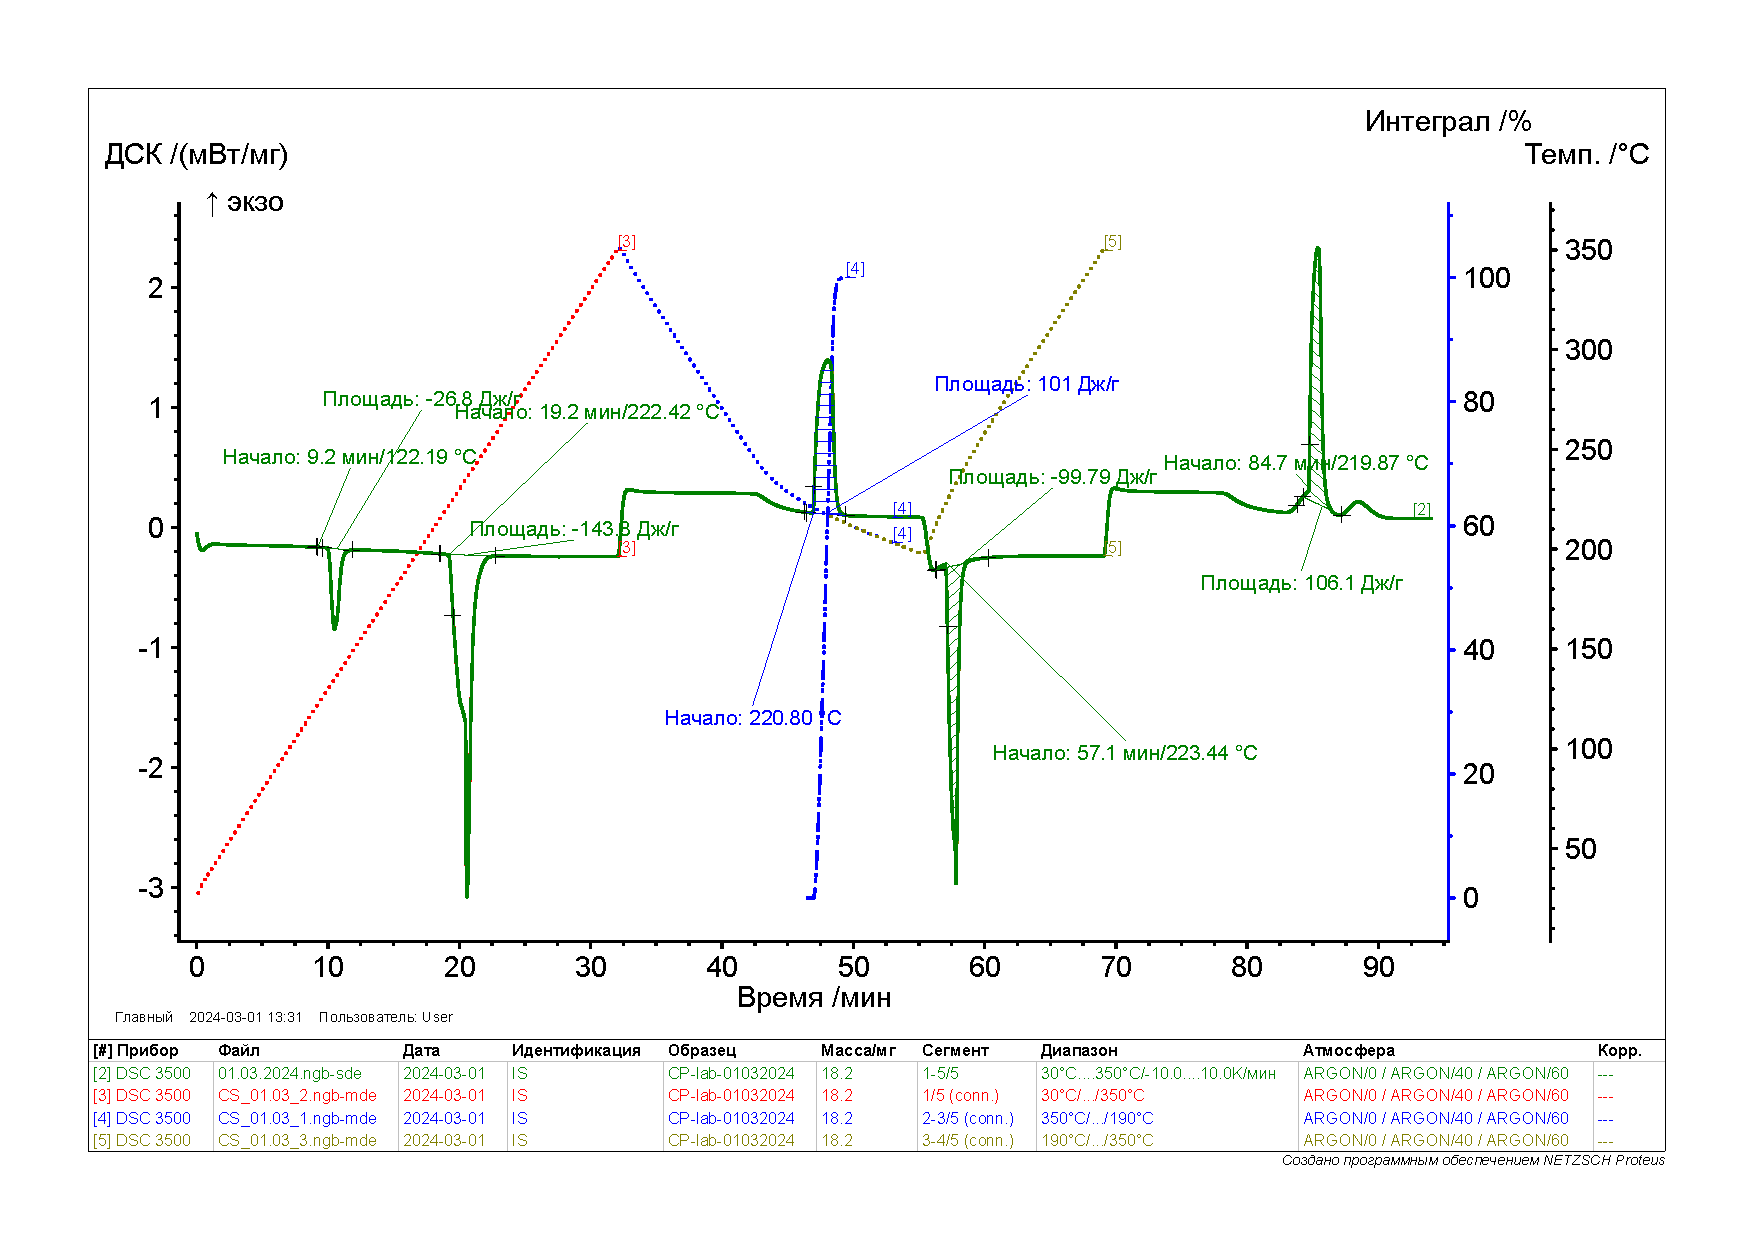
\includegraphics[width = 180 mm]{image_5.pdf}
\end{figure}

\quad \\
\\ Компоненты системы ограничено растворимы в твердом состоянии и имеются области сосущ - ия твердых растворов ${KNO}_3$ в ${NaNO}_3$ и ${NaNO}_3$ в ${KNO}_3$.
\\ Сначала наблюдаем 1-ый пик - полиморфный переход ${KNO}_3$ ($ T \approx 122.19 $°C); затем: (фазовый переход твердое - жидкое)
\\ B: $T_B$ = 222.42°C - начало плавления эвтектики;
\\C: $T_C$ = 220.80°C - начало кристаллизации при охлаждении;
\\Следующий пик получился не совсем корректным (скорее всего не дождались окончания кристаллизации) - начало кристаллизации должно было было совпасть с началом плавления.
\\D: Начало плавления $T_D$ = 223.44°C;
\\E: Начало кристаллизации $T_E$  = 219.87°C;
\\Видим, что $T_{crystallization}$ отличается от $T_{melting}$. Это может быть связано с недостаточно медленным нагревом/охлаждением. 
\\ Также были посчитаны тепловые эффекты (интегралы):
\\ $\Delta_{{crystallization}_1}$ H = 101.0 J/g;
\\ $\Delta_{{crystallization}_2}$ H = 106.1 J/g;
\\ $\Delta_{{melting}_1}$ H = -143.9 J/g;
\\ $\Delta_{{melting}_2}$ H = -99.79 J/g.
\quad \\ 
\\ Возьмем для расчетов $\Delta_{melting_2}H$ (Ближе $\Delta_{crystallization_1}$).
\\По графику определим содержание солей (По Th 222 °C);
совершается переход Calcite + ht(Na, k) ${NO}_3$ <-> ht(Na,k) ${NO}_3$. 
\\ Итого:
\\ $w_{mol}$ (${NaNO}_3$) = 0.5 = 50 $\%$
\\ $w_{mol}$ (${KNO}_3$) = 0.5 = 50 $\%$
\\\begin{table}[H]
    \begin{center}
        \begin{tabular}{|c|c|c|}
        \hline
           Вещество & $T_{melting}$, °C & $\Delta_{{melting}}$ H, kJ/mol \\\hline
          ${NaNO}_3$ & 308 & 15.09 \\\hline
          ${KNO}_3$ & 335 & 9.80 \\\hline
        \end{tabular}
        \caption{Табличные значения}
    \end{center}
\end{table}
\paragraph{Счет:}
\begin{equation}
    \ln{x} = -\frac{\Delta_{melt} {H_i}^{o}}{R}(\frac{1}{T}-\frac{1}{{T_i}^{o}}) 
\end{equation}
\\где ${T_i}^{o} = T_{melt}$; T - температура фазового равновесия

\paragraph{{NaNO}_3:}
\begin{equation}
    \ln{0.5} = -\frac{\Delta_{\melti}{H_i}^{o}}{8.31}(\frac{1}{273+223} - \frac{1}{273+308}) = 19526 (J/mol) 
\end{equation}

\paragraph{{KNO}_3:}
\begin{equation}
        \ln{0.5} = -\frac{\Delta_{\melti}{H_i}^{o}}{8.31}(\frac{1}{273+223} - \frac{1}{273+335}) = 15509 (J/mol)
\end{equation}
\paragraph{Сравнение энтальпий:}
\quad \\ Энтальпия плавления для смеси: -191.6 Дж/г (Из верхних формул) , из графика: -121.81 Дж/г.
\section{Вывод}
\quad \\ В ходе лабораторной работы были получены кривые охлаждения и нагревания $\Delta Q(t)$, $T(t)$ с помощью ДСК. По начальным температурам кристаллизации и плавления были определены фазы, в которых вещества находятся в равновесии, а также процентное соотношение веществе в смеси.
\\
\quad \\ $T_{melting}$ = 222.93 °C; $T_{crystallization} $ =  220.34 °С. 
\\
\quad \\ И по уравнению Шредера найдены удельные энтальпии плавления отдельных веществ, но результат не совпал с табличным .(Для ${NaNO}_3$: 19.5 кДж/моль; ${KNO}_3$: 15.5 кДж/моль)
\\
\quad \\Табличные значения стандартной энтальпии образования ${NaNO}_3$ и ${KNO}_3$ соотвественно равны 15.09 кДж/моль и 9.8 кДж/моль.
\\
\quad \\ Также по графику определены тепловые эффекты (энтальпии плавления смеси) ${\Delta_{mlt} H}^{o}({KNO}_3 + {NaNO}_3)$ = -99.79 Дж/г, но получили: -191.6 Дж/г.
\quad \\ Это связано с тем, что не выполняется свойство аддитивнности энтальпий (Так как вещества взаимодействут друг с другом). Также неточно были посчитаны мольные доли веществ.
\end{document}
